\begin{chapter}{Heteroscedastic \& Multilevel GP Emulators For Stochastic Simulators\label{Ch:Hetsml}}
\section{Introduction}
Offshore wind farms are becoming an increasingly attractive approach to the generation of clean, renewable energy \citep{Hobley2019}. In an effort to make the most of the abundance of offshore wind, offshore wind farms are being composed of increasing numbers of turbines. The turbines are harnessing new technologies and wind farms are being pushed further away from the coast into deep waters. Introducing new technologies to harsh environments (or employing standard technologies into new environments) induces a large number of uncertainties about, for example, the lifetimes of critical components, which ultimately impacts energy generation and profits. This uncertainty needs to be investigated prior to investing time and money into the development of these highly ambitious renewable energy projects. Stochastic computer modelling is a cost-effective approach to exploring future scenarios, but is not without its own challenges.
\subsection{Uncertainty in Stochastic Computer Models}
The uncertainties in offshore wind farms, and energy projects more generally, fall into two classes: aleatory uncertainties associated with hard-to-predict scenarios such as catastrophic weather events and epistemic uncertainties which include expected lifetimes of key turbine components. An approach to investigating these uncertainties is to formulate a stochastic model and a corresponding implementation as a stochastic computer simulator, such as the Athena simulator \citep{Zit13, Zit16}, which motivates this article (note that the simulator was given this name after the publication of these articles). The Athena simulator is a stochastic model of an offshore wind farm, with a focus on the early life of a wind farm (the first $5$ years of operational life; longer term predictions are also possible). Crucially, Athena can be used to investigate both types of uncertainty. Aleatory uncertainty can be investigated by repeatedly running the simulator at a given set of inputs. Epistemic uncertainty is investigated by running the simulator at values drawn from an expert elicited probability distribution. In this article we investigate the effect of manufacturing faults on the ``subassemblies'' of the turbines. In the Athena simulator, a turbine is constructed from $9$ subassemblies. They are the gearbox, generator, frequency converter, transformer, main shaft bearing, the blades, tower, foundations. There is also a ninth `catch all' subassembly which captures all the other turbine components, which individually have a very minor impact on wind farm performance, but jointly could have more serious implications on wind farm performance. We denote the expected subassembly lifetimes by $\{x_1, x_2, \ldots, x_9\}$, where the ordering $1$--$9$ reflects the order in which subassemblies have been listed above (including the catch all). Subassembly failures conditional on a manufacturing fault in subassembly $i$ occur according to an $Exp(1/x_i)$ distribution. The $x_i$ are unknown so are to be elicited and varied in uncertainty and sensitivity analyses.

A key model output is a time series which tracks the ``availability'' of a wind farm over time (see \Cref{Fig:availability-trajectories}). Availability is a measure of reliability (performance) of offshore wind farms; the availability at time $t$ is the energy output of the wind farm as a proportion of the maximum possible energy output at time $t$. In this article we compress the availability time series into a single value --- the average availability. This is the mean availability over the simulation period. Offshore wind farms reach an availability of around $93\%$ for near shore turbines, but this is reduced for turbines further away from the coast since reaching the turbines for repair is much more difficult \citep{Carroll2016}. Availability is related to a wind farm's uptime and hence its profitability.
\begin{figure}[h]
	\centering
	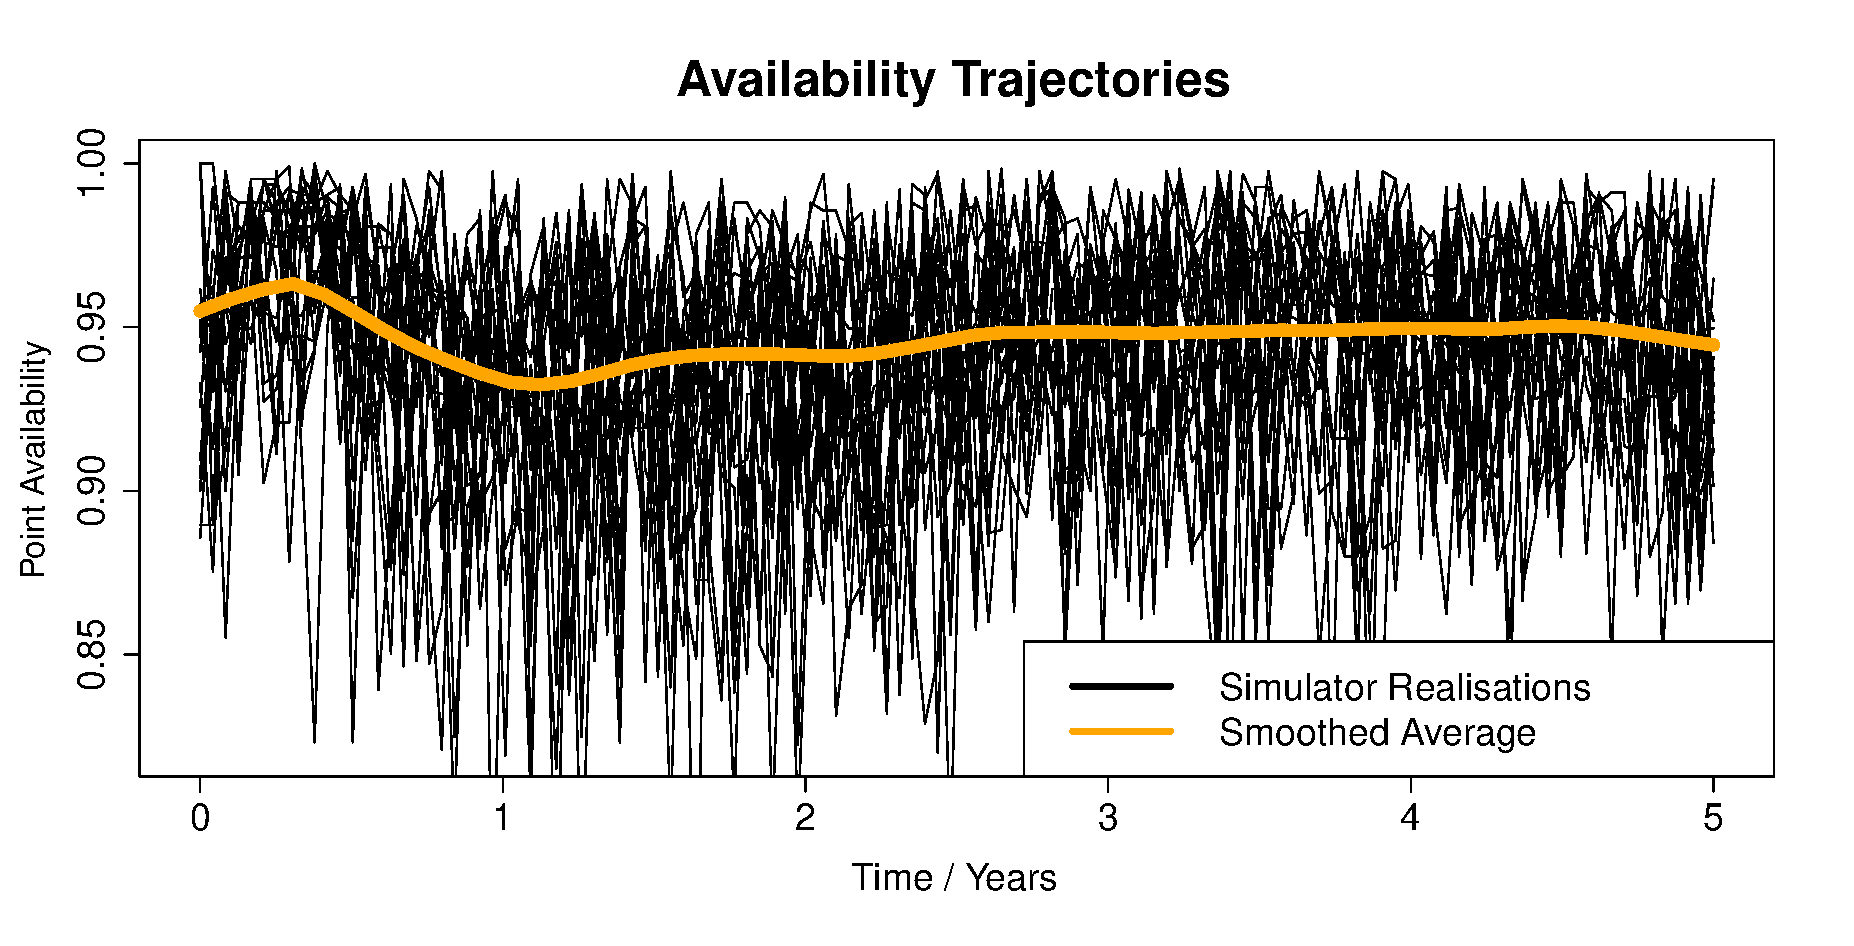
\includegraphics[width = 0.75\textwidth]{sml-het-fig/avail-traj-years.eps}
	\caption{A collection of $10$ availability trajectories (black lines) over the first $5$ years of a wind farm's operational life for a fixed set of parameter values. The orange line represents a smoothed average of the trajectories.}
	\label{Fig:availability-trajectories}
\end{figure}
%% some information about the athena simulator
The Athena simulator is a point processes model which simulates events at discrete times over a time period $[0, T_{max}]$. Events are usually a component in the wind farm breaking or being repaired, but can, for example, be the triggering of farm-wide maintenance or the deployment of a boat to perform a repair. To simulate events, the simulator starts from time $t=0$ and calculates the hazard function of each event at each time point over the period of interest; this is a function of time and the state of the wind farm. From this the ``total'' hazard (at each time point), known as the Force of Mortality (FOM), is calculated which then implies the next event time. This time is found as the solution to an integral, which is solved numerically. The individual hazards of each wind farm component also imply the probability of the event being associated to that particular component at the new event time. These are calculated as the hazard for the particular event divided by the FOM. These probabilities form a partition of $[0,1]$ so a $U(0,1)$ random variable is drawn. If the random variable falls in the partition associated to a given event, then that is the event that occurs. This is repeated until we reach the end of the pre-specified simulation period $T_{max}$.

 In our simulations $T_{max} = 5$ (years); the early life in which \textit{excessive failure} is frequently observed. That is, the wind farm typically under-performs due to more than expected numbers of component failures; tackling this issue is vital to the feasibility of offshore wind. The number of event times is affected by a tuning parameter $\Delta t$, which represents the length of the time step of the numerical integration in the simulator which finds the (random) time between events. If $\Delta t$ is too large then we will frequently over estimate the time at which an event occurs, which results in an inaccurate simulation. Decreasing $\Delta t$ gives more accurate simulations but at an increased computational cost. Accurate runs of the Athena simulator take approximately $11$ minutes for a wind farm with $200$ turbines. For reference, the world's largest offshore winds farms (measured by number of turbines) are the London Array with $175$ turbines and the Hornsea $1$ which has $174$ \citep{Paterson2018, Vanhellemont2014}.

The purpose of the Athena simulator is decision support under uncertainty. These uncertainties being the epistemic uncertainty an expert would have about parameters of a simulator and the aleatory uncertainty about the natural world, for instance, the weather and the implications this has on wind farm performance. An engineer designing the wind farm may be able to choose between a ``tried and tested'' component or a new component with a novel design. This could be a choice between one of two gearboxes for the turbine. The engineer would (with the help of a facilitator) formulate uncertainty distributions over the performance of each gearbox (for example, expected component lifetime) and then propagate this uncertainty through the Athena model to see how the uncertainty in component performance impacts wind farm performance. When there is just one uncertain parameter to elicit, we can spend all available resources (time, money, patience of experts) on eliciting a probability distribution for this parameter. When many uncertain parameters are of interest, the finite nature of our resources becomes very real. Therefore, as per the Sheffield Elicitation Framework (SHELF) protocols, we need to identify which parameters are most important to the problem at hand. We then perform a full SHELF workshop on the parameters deemed most important. We employ less precise probability judgements on less critical parameters \citep{SHELF4}. Putting this into the context of eliciting parameters for a complex computer model, it is not clear which parameters are most important until a sensitivity analysis has been conducted. Probabilistic sensitivity analysis (PSA) will be our approach to tackling this problem of parameter importance; PSA allows us to quantify the proportion of output uncertainty (measured by variance) induced by any input (or even groups of inputs). The most important inputs are those contributing the most to output uncertainty \citep{Oakley04}.

A bottleneck we encounter is that the Athena simulator is computationally expensive. It will be computationally infeasible to perform PSA to understand the influence of key parameters on wind farm performance. Further, the stochastic nature of the model makes these computations even more cumbersome. It is common in such scenarios to build a statistical surrogate model --- an \emph{emulator} --- to replace the simulator \citep{Gramacy2020surrogates}. The Monte Carlo calculations to perform PSA become very manageable with an emulator \citep{Marrel2012}. The theory of emulation of deterministic models is well developed, dating back to at least \citet{Sacks89}. Emulation has been applied to a broad range of scenarios such as, but not limited to, calibration \citep{Ohagan01}, uncertainty/sensitivity analysis \citep{Kennedy2006} and optimisation \citep{Wilson2018}.

\subsection{Emulators}

One of the most powerful approaches to emulation (of deterministic simulators) is to construct a Gaussian Process (GP) emulator, although other types of surrogate are available; see, for example, \citet{Goldstein2006,Sudret2008, Rougier2010}. From the Bayesian perspective, an emulator is constructed by first assuming a GP prior distribution over the simulator outputs. Runs of the model, known as training data, are used to update beliefs about the value of the unknown function at (untried) inputs. These updated beliefs are represented as a posterior probability distribution. An alternate approach is to view the emulator as a Kriging predictor for the output of the simulator at untried inputs \citep{Sacks89}. Once constructed, emulators produce fast predictions of simulator output at untried inputs. The computational burden of running the simulator is frequently reduced by several orders of magnitude when replaced by an emulator. What makes emulators favourable to other surrogates is the quantification of (epistemic) uncertainty attached to the prediction \citep{Ohagan2006}.

More recently, as \emph{stochastic} simulation has become more prominent, so has the interest in the emulation of stochastic computer simulators, for example, \citet{Astfalck19, Rocchetta2018, Boys2018}. There are a variety of approaches to (GP based) emulation of stochastic computer models; see \citet{Baker2020} for a recent overview. One desirable feature of many of these emulators is that they give us not only a mean response but also a quantification of both types of uncertainty in the simulators; the \emph{extrinsic} (epistemic) uncertainty which quantifies our (lack of) knowledge in mean simulator output, and the \emph{intrinsic} (aleatory) uncertainty, that is, the simulator's level of noise at any tried or untried input.

Although the stochastic setting is more familiar to the statistician, the emulation of stochastic simulators is invariably more challenging. Many GP based emulation approaches for stochastic problems rely on large levels of replication, which is a sensible procedure when the stochastic simulator is not overly expensive or a sufficiently large computing budget is available for training data. To estimate the mean response of a stochastic simulator, we might apply Stochastic Kriging (SK) to runs of the simulator \citep{Akenman2010}. For SK it is recommended that we use at least $10$ replicates at each design point. If we require a surrogate for the noise, a pair of GP emulators (one for the mean, another for the noise) can be constructed as in \citet{Henderson09}, who use around $1000$ replicates per design point; a similar approach is used by \citet{Andrianakis2017}. Another input dependent noise formulation is Quantile Kriging \citep{Plumlee2014}, which again uses replication -- hundreds of replicates are required to model non-Gaussian, input dependent, noise in computer simulators.  The Athena model can take up a prohibitive amount of time for a single accurate run, thus such levels of replication would make emulation of the Athena model infeasible. It is also likely that for many problems, a simple transformation could remedy any asymmetry in a simulator's output distribution.

An approach which need not require replication, but still allows for it, is the heteroscedastic GP (HetGP) \citep{Goldberg1998, hetGP}. The allure of HetGP is the promise of a full surrogate; joint prediction of the mean response and the level of noise at any input combination. This is possible via a latent variable formulation which jointly models the simulator mean as a GP and the log noise (to ensure positivity) as a GP. As \citet{Gramacy2020surrogates} notes, this coupled GP approach provides smooth estimates of the noise at both within sample and out of sample simulator inputs. However, this very flexible approach to emulation may still require prohibitively large sample sizes to produce a satisfactory emulator. For example, \citet{Binois2018} use $500$ design points to compare emulators for a one dimensional stochastic simulator.

In the Athena simulator it is simple to change model features to give us cheap approximations to large offshore wind farms. Since these approximations are relatively computationally cheap, it is easy to get enough training data to construct good emulators. If we can build a good emulator for the cheap simulator, and accurately describe its mean, perhaps we can utilise this information to build better emulators for more expensive stochastic computer models.

Exploiting cheap approximations to an expensive simulator has been tackled in the deterministic framework by \citet{Kennedy2000}. The most popular format is their autoregressive structure for functions \citep{Forrester2007, Singh2017, Harvey2018}. The autoregressive structure builds a well informed emulator for the cheap simulator and use this as a ``starting point'' for the expensive simulator. The main aim of multilevel emulation is an improved emulation of the (expensive) simulator at a fixed training budget. We aim to extend this to the more complex case of stochastic computer experiments to enhance the emulation of the Athena simulator.% Related work, Stochastic Co-Kriging (SCK), is given by \citet{Chen2017}, however their surrogate is a variant on Stochastic Kriging which is aimed at producing a mean response surface and typically requires large amounts of replication. We will focus on a replication-free framework; using the latent variance formulation of HetGP.

%% --- paper structure ---
The remainder of the article is structured as follows. Section $2$ outlines emulation via heteroscedastic Gaussian processes. In Section $3$ we motivate and propose stochastic multilevel emulation, which is a key contribution of this article. Section $4$ describes a short simulation study. We return to the Athena model in Section $5$ where a stochastic multilevel emulator is produced and validated. Probabilistic sensitivity analysis using our proposed emulation method is performed in Section $6$. Section $7$ contains concluding remarks.

\section{Heteroscedastic Gaussian Processes (HetGP)}

Here we outline HetGP \citep{Binois2018} to later draw parallels with Stochastic Multilevel (SML) emulation. Suppose we have a complex stochastic simulator, $\eta(\cdot)$. We can model this as a heteroscedastic GP:
\begin{align*}
\eta(\cdot) | \lambda^2(\cdot) &\sim  \mathcal{GP} \{ m(\cdot), C(\cdot, \cdot) + \lambda^2(\cdot) \}\nonumber \\
\log \lambda^2 (\cdot) &\sim  \mathcal{GP} \{ m_V (\cdot), C_V (\cdot, \cdot) + \lambda_{V}^2 ) \}.\nonumber
\end{align*}
\noindent Here, $m(\cdot)$ and $m_V(\cdot)$ are prior mean functions. These mean functions are typically expressed in a hierarchical form such as $m(\bx) = h(\bx)^T \bm{\beta}$, where $\bx$ is the $K$ dimensional simulator input, $h$ a collection of simple, deterministic basis functions and $\bm{\beta}$ are unknown coefficients of the basis functions to be inferred. The mean function on the log-variance $m_V(\cdot)$ is expressed similarly; $m_V(\bx) = h_V(\bx)^T \bm{\beta}_V$. Here, $\lambda^2(\cdot)$ is the (aleatory) uncertainty of the expensive simulator; the log of this is modelled by a GP which itself has aleatory uncertainty $\lambda^2_V$. Since the noise (and therefore covariance function) depends on $\bx$, HetGP is a type of non-stationary GP.
% These noise terms, especially for constant $\lambda$, are sometimes referred to as a ``nugget'' effect \citep{Gramacy12}.

 Similarly, we parameterise $C$ and $C_V$, the covariance functions. A common choice of covariance function for computer experiments is the \emph{squared exponential} covariance function, as this imposes the belief that the moments of the simulator output are smooth functions of the simulator inputs \citep{Santner2003}. A squared exponential covariance function, for a simulator with $K$ inputs, is of the form $C(\bx, \bx') = \sigma^2 \exp \left\{  -(\bx - \bx')^{T}D^{-1}(\bx - \bx') \right\}$, where $\sigma^2$ is a scale parameter and $D = \text{diag}(\theta_1 ^2, \ldots, \theta_K ^2)$ is a diagonal matrix of correlation lengthscales. The same form is given to $C_V$, but the scale ($\sigma_V^2$) and lengthscale parameters ($\theta_{k, V})$ can take different values.

We then run the simulator $n$ times to obtain training data $\mathcal{D} = \{y_i, \bx_i : i = 1, \ldots, n\} $, where $y_i$ are single runs/realisations of $\eta(\bx_i)$. The hyperparameters, \newline $\Theta = \{\theta_1, \ldots, \theta_K, \theta_{1,V}, \ldots, \theta_{K,V}, \bm{\beta}, \bm{\beta}_V, \sigma, \sigma_V, \lambda_{V} \}$, can then be inferred and the log variance, $\log \lambda^2(X) = \left( \log \lambda^2(\bx_1), \ldots, \log \lambda^2(\bx_n) \right)$, at the design points, $X = \{\bx_1, \ldots, \bx_n \}$, can also be estimated. Conditional on $\mathcal{D}$, $\Theta$, and $\log \lambda^2(X)$, the posterior predictive distribution of the intrinsic variance at a new input $\bx^\star$ is
\begin{equation}
\log \lambda^2(\bx^\star) | \log \lambda^2(X), \mathcal{D}, \Theta \sim \mathcal{N} \left\{ m_V^\star(\bx^\star), C_V^\star(\bx^\star, \bx^\star) + \lambda_{V}^2 \right\}. \nonumber
\end{equation}
where the posterior moments are found via the conditional normal equations,
\begin{align}
m^\star_V(\bx^\star) & = m_V(\bx^\star) + C_V(\bx^\star, X)
\left[C_V(X, X) + \lambda_{V}^2 I_n \right]^{-1}\left(\log \lambda^2(X) -  m_V(X) \right) \nonumber\\
C_V^\star(\bx^\star, \bx^\star) & = C_V(\bx^\star, \bx^\star) - C_V(\bx^\star, X) \left[C_V(X, X) + \lambda_{V}^2 I_n \right]^{-1}C_V(X, \bx^\star)\nonumber
\end{align}
and $I_n$ is the $n \times n$ identity matrix.
Then conditional on the data, and hyperparameters, the posterior predictive distribution of the simulator output at an input $\bx^{\star}$ is
\begin{equation}
\eta(\bx^\star) | \Theta, \mathcal{D} \sim \mathcal{N} \left\{ m^\star(\bx^\star) , C^\star (\bx^\star, \bx^\star) + \lambda^{\star 2} (\bx^\star) \right\}.\nonumber
\end{equation}
Here, $\lambda^{\star 2} (\bx^\star) = \exp\{ m_V ^\star (\bx^\star) \}$ and $m^\star(\bx^\star)$, $C^\star (\bx^\star, \bx^\star)$ are also found by the conditional normal equations:
\begin{align}
m^\star(\bx^\star) & = m(\bx^\star) + C(\bx^\star, X) \left[ C(X,X) + \lambda^{\star 2} (X) I\right]^{-1}\left( \bm{y} - m(\bx) \right) \nonumber \\
C^\star(\bx^\star, \bx^\star) & = C(\bx^\star, \bx^\star) -  C(\bx^\star, X) \left[ C(X,X) + \lambda^{\star 2} (X) I \right] ^{-1} C(X, \bx^\star) \nonumber
\end{align}
where $\bm{y} = (y_1, \ldots, y_n)^T$.

In \Cref{Fig:toy-HetGP} we see an example HetGP emulator for the stochastic simulator $\eta(x) = 4\sin(6 \pi x) + 5x + (1.1+7x)\varepsilon$ where $\varepsilon \sim \mathcal{N}(0,1)$.
\begin{figure}[h]
	\centering
	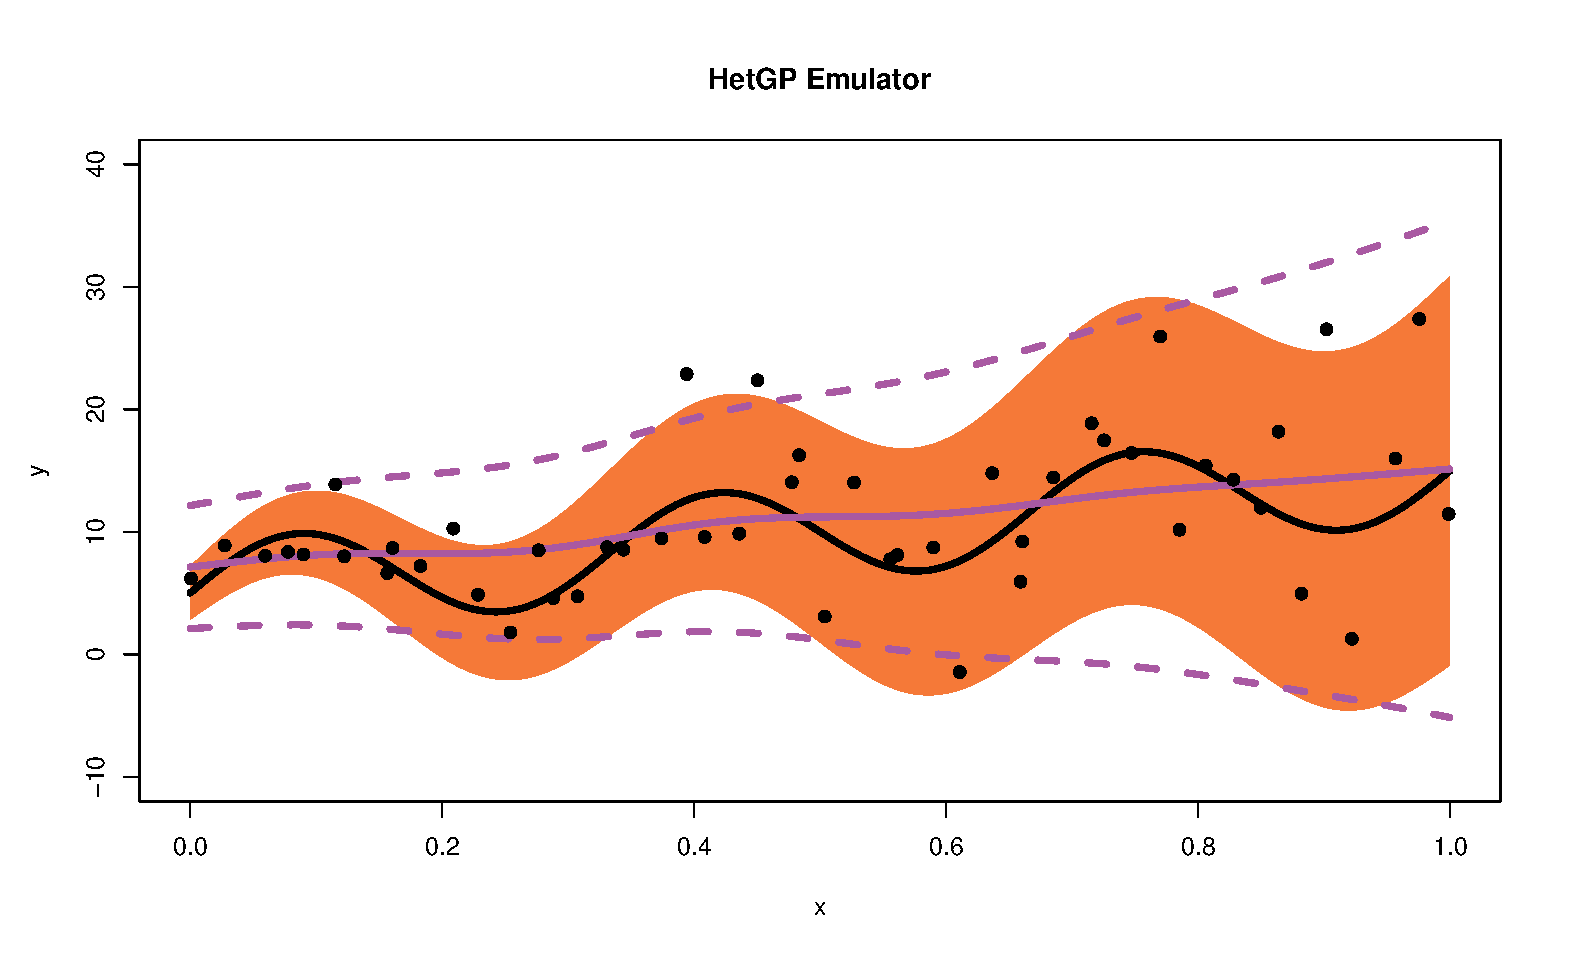
\includegraphics[width=0.75\textwidth]{sml-het-fig/hetgp-example.eps}
	\caption{A HetGP emulator for $\eta(\cdot)$. Black points are the outputs from $50$ runs of the simulator. Black line represents the true simulator mean and the orange band represents the mean $\pm 1.96$ `true' standard deviations. Solid purple line represents emulator mean with dashed lines being the emulator mean $\pm 1.96$ emulator standard deviations.}
	\label{Fig:toy-HetGP}
\end{figure}
Observing the fit in \Cref{Fig:toy-HetGP}, the fitted emulator mean (purple lines) does not match up well with the simulator. The emulator predicts an approximately linear response whereas the simulator is clearly sinusoidal in nature. The emulator is interpreting the systematic sinusoidal variation as noise, rather than signal. Ultimately, this is because emulating a stochastic computer model requires much more information than the standard deterministic problem. However, when provided with adequate amounts of data, HetGP can produce excellent surrogates for complex stochastic computer models \citep{Binois2018}.

\section{Stochastic Multilevel Emulation}

\subsection{Motivation and Intuition}


We outline our proposed approach to stochastic multilevel (SML) emulation which naturally extends deterministic emulation techniques and exploits the cheap approximations that are readily available from the Athena simulator. This approach is quite general and will apply to many stochastic simulators when cheap approximations are available. Many stochastic computer simulators have a complexity parameter, such as the length of a time step, or granularity of a grid over space, which exchanges simulation accuracy for computational efficiency, examples include \cite{Kennedy2000} and \citet{Le2014}. In our wind farm setting this will be the `time step' in a numerical integration within each simulation run, as well as the overall wind farm size (number of turbines). The accuracy required comes at a computational cost which severely hinders the size of our computer experiment, limiting the quality of the fitted emulator and future inferences. We aim to exploit such properties in jointly modelling the ``cheap'' simulator and ``expensive'' simulator. The outputs from cheap and expensive versions of stochastic simulators will be related. Runs from both versions will be combined to build an overall better emulator.

We will focus on a two level set up;  $\eta^C(\cdot)$ is the cheap simulator and $\eta^E(\cdot)$ is its expensive counterpart. In the motivating example of the Athena model $\eta^C(\cdot)$ is a version of the model with $50$ turbines and a time step of $\Delta t = 0.1$ years (simulating time steps of just over a month). However, we want to infer $\eta^E (\cdot)$, which is a version with time step $\Delta t = 0.001$ years (simulating time steps of approximately $9$ hours) and $200$ turbines.

\subsection{Proposed Emulation Strategy}
Here we will present our stochastic multilevel emulator. We allow for $\eta^E(\cdot)$ to be heteroscedastic but if we believe it is homoscedastic we can replace the non-constant variance with a constant term. Our object of inference is (the distribution of) $\eta^E(\bx)$, for any $\bx$.

Suppose that the cheap simulator, $\eta^C(\cdot)$ can be modelled by a homoscedastic (constant noise) GP with mean function $m_C(\cdot)$, covariance function $C_C(\cdot, \cdot)$ and constant variance $\lambda^2_C$:
\begin{equation}
	\eta^C(\cdot) \sim \mathcal{GP} \left( m_C(\cdot), C_C(\cdot, \cdot) + \lambda^2_C  I\right).\nonumber
\end{equation}
We expect that the cheaper simulator's mean is somehow informative for the expensive counterpart and thus, as in \cite{Kennedy2000}, we assume that
\begin{equation}
	\eta^E(\cdot)|\rho, \E\{\eta^C(\cdot)\}, \delta(\cdot) = \rho \E\{ \eta^C(\cdot) \} + \delta(\cdot)\nonumber
\end{equation}
where $\eta^E (\cdot)$ is the expensive stochastic simulator and $\delta(\cdot)$ is a heteroscedastic GP:
\begin{align}
	\delta(\cdot)|\lambda_E^2 (\cdot) \sim \mathcal{GP}\left( m_E(\cdot), C_E(\cdot, \cdot) + \lambda^2_E(\cdot)I \right) \nonumber\\
\log \lambda^2_E(\cdot) \sim \mathcal{GP} \left( m_V(\cdot), C_V (\cdot, \cdot) + \lambda_{V}^2 I \right).\nonumber
\end{align}
In this formulation, $\rho \in \R$ is a regression parameter and $m_E(\cdot)$, $C_E(\cdot, \cdot)$ are mean and covariance functions for $\delta(\cdot)$. The term $\delta(\cdot)$ serves a dual purpose. Firstly, $\delta(\cdot)$ can be viewed as a discrepancy function; the mean of $\delta(\cdot)$ represents the difference in the mean response of the two simulators, or the loss of accuracy from running cheap simulations (with a large time step/coarse grid). Secondly, $\delta(\cdot)$ describes the stochasticity in the expensive simulator. This is a similar structure to that of Bayesian calibration of deterministic computer models \citep{Ohagan01}, however we do not observe data from a physical system --- but a computer simulator --- and we have noise in both sets of observations.

This joint model for the two simulators allows us to borrow information from the cheaper simulator, but is sufficiently flexible to reject a relationship between the two levels if no such relationship exists. Namely, if $\rho = 0$ we recover HetGP.

We express the mean functions in a hierarchical form so that
\begin{align}
	m_C(\bx) &= h(\bx)^T \bm{\beta}_C \nonumber\\
	m_E(\bx) &= h(\bx)^T \bm{\beta}_E.\nonumber
\end{align}
We take $h(\cdot)$ to be a set of known, deterministic basis functions with coefficients given by the $\bm{\beta}$ terms. A typical choice for $h(\cdot)$ is a collection of low order monomials which capture the global variation in the simulator output. A particularly common choice is $h(\bx)^T = (1, \bx^T)$ \citep{Fricker2011, Becker2012}. Hence, the mean functions have the same form, but the particular parameters of these regression functions are allowed to differ.

We will use squared exponential covariance functions so that
\begin{align}
	C_{*}(\bx, \bx') =  \sigma^2_{*} \exp\left\{ -(\bx - \bx')^T D^{-1}_{*}(\bx -  \bx')\right\}\nonumber
\end{align}
\noindent where $* \in \{C, E\}$, $D_{*} = \diag(\theta_{1, *}^2, \ldots, \theta_{K, *}^2)$ is a diagonal matrix containing the correlation lengthscales and $\sigma_*$ are scale parameters of the covariance functions. The choice of a squared exponential covariance function is imposing the belief that the mean and variance of the simulator are smooth and infinitely differentiable. Note that the choice  of squared exponential covariance function is not a requirement, the user can specify a different covariance structure as they see fit \citep{Rasmussen2006}.


Hence a hierarchical model for the expensive simulator is as follows:
\begin{align*}
	\eta^E(\cdot) | \rho, \E\{ \eta^C(\cdot) \}) & = \rho \E\{ \eta^C(\cdot) \} + \delta(\cdot)\nonumber \\
	\eta^C(\cdot)  & \sim \mathcal{GP} \{ m_C(\cdot), C_C(\cdot, \cdot) + \lambda^2_C I_C\}\nonumber\\
	\delta(\cdot)|\lambda_E^2(\cdot) & \sim  \mathcal{GP} \left\{ m_E(\cdot), C_E(\cdot, \cdot) + \lambda^2_E(\cdot) I_E  \right\}\nonumber \\
	\log(\lambda_E^2(\cdot)) &  \sim \mathcal{GP} \left\{ m_V(\cdot), C_V (\cdot, \cdot) + \lambda_{V}^2 I_E \right\},\nonumber
\end{align*}
where $\lambda_C$ is a constant nugget effect for the cheap simulator. Since we are only interested in the cheap simulator's mean, we do not feel that it is necessary to estimate a surface for its variance. In fact, \citet{Binois2019} observe that a homoscedastic GP is quite good at learning the mean response surface, even in the face of heteroscedasticity (see Fig. $5$ of \citep{Binois2019}). Here, $\lambda_{V}$ is a constant nugget effect for the latent variance of the expensive simulator. Both $\lambda_C$ and $\lambda_V$  smooth the noisy simulator observations. The $I_{*}$ are identity matrices of appropriate dimensions. Hence a SML emulator has a similar structure to the standard multilevel emulators presented by \cite{Kennedy2000}, with the addition of a latent variance process ($\lambda_E^2(\cdot)$). We model the log variance as a GP to enforce positivity.

It follows that, conditional on all hyperparameters,\newline $\bm{Y}^T = \left( (\bm{Y}^C)^T, (\bm{Y}^E)^T \right)= (Y^C_1, \ldots, Y^C_{N_C}, Y^E_1, \ldots, Y^E_{N_E})^T$ are multivariate normal where $N_C$ and $N_E$ are the number of runs of the cheap and expensive simulators, respectively. That is
\begin{equation*}
\begin{pmatrix} \bm{Y}^C \\ \bm{Y}^E \end{pmatrix} \sim \mathcal{N}_{N_C + N_E} \left\{ \begin{pmatrix} m_C(X^C) \\ \rho m_C(X^E) + m_E(X^E) \end{pmatrix}, \var(\bm{Y}) \right\}
\end{equation*}
where $X^C$ and $X^E$ are the design matrices of the cheap and expensive codes, respectively. Further details of the design are given in \Cref{Sec:design}.

We will now derive the covariance matrix of the response $\bm{Y} = (Y^C_{1}, \ldots, Y^C_{N_C}, Y^E_{1}, \ldots, Y^E_{N_E} )^T$. We express this covariance matrix in block form so that
\begin{equation}
\var(\bm{Y}) = \begin{pmatrix}
\var(\bm{Y}^C) & \cov(\bm{Y}^C, \bm{Y}^E) \\
\cov(\bm{Y}^E, \bm{Y}^C) & \var(\bm{Y}^E)
\end{pmatrix}.\nonumber
\end{equation}

The auto-covariance of $\bm{Y}^C$ is
\begin{equation*}
\var(\bm{Y}^C)_{i,j} = \sigma^2_C \exp \left\{ -(\bx_i - \bx_j)^T D^{-1}_C (\bx_i - \bx_j)\right\} + \lambda_C^2 \mathbb{I}_{\bx_i, \bx_j},\nonumber
\end{equation*}
\noindent where $\mathbb{I}_{i, j}$ is an indicator function equal to $1$ when $i=j$ and $0$ otherwise. For the auto-covariance of the expensive simulator, we assume the three summed GPs are all pairwise independent and that the constant variance of the cheap simulator is independent of the variance of the expensive simulator. Further we assume, for $i \neq j$ that
\begin{align*}
\cov(Z^C(\bx_i), \delta(\bx_j)) &= 0\nonumber \\
\cov(Z^C(\bx_i), \lambda^2_E(\bx_j)) &= 0\nonumber \\
\cov(\delta(\bx_i), \lambda^2_E(\bx_j)) &= 0,\nonumber
\end{align*}
where $Z^C(\bx)$ is shorthand for $\E\{ \eta^C(\bx) \}$. Thus we find that:
\begin{align*}
\var(\bm{Y}^E)_{i,j} & = \cov(Y^E(\bx_i), Y^E(\bx_j))\nonumber\\
 & = \cov\left( \rho Z^C(\bx_i) + \delta(\bx_i) + \varepsilon^E_i(\bx_i), \rho Z^C(\bx_j) + \delta(\bx_j) + \varepsilon^E_j(\bx_j)\right) \nonumber\\
%& =  \rho^2 \cov(Z^C(\bx_i), Z^C(\bx_j)) + \cov(\delta(\bx_i), \delta(\bx_j)) + \cov(\varepsilon^E_i(\bx_i), \varepsilon^E_j(\bx_j))\nonumber \\
%& = \rho^2 \sigma^C^2 \exp\left\{ -(\bx_i - \bx_j)^T D^{-1}^C (\bx_i - \bx_j) \right\} \nonumber\\
& \hspace{1cm} + \sigma_E^2 \exp\left\{ -(\bx_i - \bx_j)^T D^{-1}_E (\bx_i - \bx_j) \right\}  + \lambda^2_E(\bx_i)\mathbb{I}_{\bx_i, \bx_j}\nonumber
\end{align*}
where the $\varepsilon^E_i(\bx_i)$ represents the input dependent noise in the expensive simulator with input vector $i$ and $\varepsilon^C_j$ is the (assumed) constant noise exhibited in the cheap simulator at input vector $j$. Finally, the cross-covariance is given by
\begin{equation*}
\cov(\bm{Y}^C, \bm{Y}^E)_{i,j}  = \rho \sigma^2_C \exp \left\{ -(\bx_i - \bx_j)^T D^{-1}_C (\bx_i - \bx_j)\right\}.
\end{equation*}
\subsection{Prior Specification}


Since a Bayesian approach to inference is adopted, we assign priors to all GP parameters. We propose that all parameters are assumed independent \textit{a priori} with the following distributions (where the hyperparameters of the prior are chosen by the user):
\begin{align}
\beta_{j, *} &\sim \mathcal{N}(m_{j,*}, s_{j,*}^2)\nonumber \\
\theta_{j,*} &\sim  Gamma(a_{j, *}, b_{j, *}) \nonumber\\
\sigma_* &\sim Inv-Gamma(c_{j,*}, d_{j,*}) \nonumber\\
\lambda_*^2 &\sim Inv-Gamma(e_{j,*}, f_{j,*})\nonumber \\
\rho &\sim \mathcal{N}(m_{\rho}, s_{\rho}^2),\nonumber
\end{align}
\noindent where $* \in \{C, E, V \}$. Note that there is no $\lambda^E$ since we replace this by a GP to account for heteroscedasticity. We adopt priors over the $\beta^{*}_j$ that are very flat, as is often the case in the computer experiments literature \citep{Oakley2017}. Hence we take $m_{j,*} = 0$ and $s_{j,*}=10$. Our priors on $\theta_{*}$ will be reasonably uninformative, but designed to omit very large lengthscales, therefore we take $a_{j,*} = 2$ and $b_{j,*} = 1$. Again, fairly weak priors are taken over $\sigma_*$; $c_{j,*}=d_{j,*}=2$ and for $\lambda^2_*$ we have $e_j = f_j=2$. However, in the prior for $\rho$ we are being quite subjective, we take $m_\rho = 1$ and $s_\rho = 1/3$. This specification expresses the belief that the codes are positively correlated with a high probability; this is a reasonable assertion. If this belief was not held, then there would be little reason to construct a multilevel emulator. This specification is \textit{our} prior specification. In practice, a user can choose a prior that they see suitable.

We will use this same prior specification throughout the paper, but when the input space has dimension $\geq 2$ we model $\theta_{i, *}$ via independent $Gamma(2,1)$ priors.

\subsection{Design \label{Sec:design}}

We require a space filling design for both the cheap and expensive versions of the simulator, hence we will appeal to a nested design based on Latin Hypercubes. We generate $X^E$ via a Maximin Latin Hypercube \citep{Mckay1979} (using the \verb|lhs| package in \verb|R|). To generate $X^C$ we make another Maximin Latin Hypercube and append the two designs together. Note that we will run the both the cheap and expensive version of the simulator at $X^E$, but only run only the cheap simulator at $X^C$.

\subsection{Posterior Predictive Distribution of Code Output}
Within our Bayesian approach, \textit{maximum a posteriori} (MAP) estimates will be used as point estimates of the parameters.  In practice, we find the MAP estimates via a numerical optimisation of the log-posterior (up to an additive constant) using the \verb|optimizing| function from rstan \cite{stan}. This is not fully Bayesian, however it is computationally thrifty. Markov chain Monte Carlo allows for a full Bayes analysis but \cite{Kersting2007} note a full Bayes analysis is very computationally expensive for standard Gaussian Process regression problems, let alone our more complicated variant.

Conditional on point (MAP) estimates, and estimates of the log variance at the design points, prediction of the log variance is the same as for HetGP, that is, Gaussian with mean
\begin{equation*}
m^\star_V (\bx) = m_V(\bx) + C_V(\bx, X^E) \big\{ C_V(X^E, X^E) + \lambda_{V}^2 I_E \big\} ^{-1} (\log (\lambda^2_E(X^E)) - m_V(X^E) )\nonumber
\end{equation*}
and variance
\begin{equation*}
v^\star_V(\bx) = C_V(\bx, \bx) + \lambda^2_V - C_V(\bx, X^E) \big\{ C_V(X^E, X^E) + \lambda_{V}^2 I_E \big\} ^{-1} C_V(X^E, \bx).\nonumber
\end{equation*}
Prediction of the simulator mean at input $\bx$ is more complex, but is a natural extension of the posterior predictive mean of a two-level code given in \cite{Kennedy2000}. Having observed code outputs $\bm{Y}^C$, $\bm{Y}^E$ at design points $X^C$, $X^E$, our design matrix is
\begin{equation}
H = \begin{pmatrix}
h(\bx^C_1)^T & \bm{0} \\
\vdots & \vdots \\
h(\bx^C_{N_c})^T & \bm{0} \\
 & \\
\rho h(\bx^E_1)^T & h(\bx^E_1)^T \\
\vdots & \vdots \\
\rho h(\bx^E_{N_E})^T & h(\bx^E_{N_E})^T
\end{pmatrix}\nonumber
\end{equation}
and hence the posterior distribution of the output of the expensive simulator at a new input $\bx$, conditional on a point estimate of the hyperparameters, is Gaussian with mean
\begin{equation}
m^\star(\bx) = h_0(\bx)^T \bm{\beta} + t(\bx)^T \var(\bm{Y})^{-1}(\bm{Y} - H\bm{\beta})\nonumber
\end{equation}
 and variance
\begin{equation}
V^\star(\bx) = V(\bx) - t(\bx)^T \var(\bm{Y})^{-1} t(\bx),\nonumber
\end{equation}
where
\begin{align}
h_0(\bx) &= (\rho h(\bx)^T, h(\bx)^T)^T\nonumber \\
\bm{\beta} &= \left( \bm{\beta}_C ^T, \bm{\beta}_E ^T \right)^T\nonumber \\
t(\bx)^T &= \left( \rho \cov(Z^C(\bx), Z^C(X^C)), \rho^2_ \cov(Z^C(\bx), Z^C(X^E) + \cov(\delta(\bx), \delta(X^E)) \right) \nonumber\\
V(\bx) & = \rho^2 C_C(\bx, \bx) + C_E(\bx, \bx) + \lambda_E^2(\bx) .\nonumber
\end{align}

\section{Simulation Study\label{Sec:simulation-studies}}
\subsection{ Emulator Comparison \label{Sec:testing-method}}

Before we apply SML to the Athena model, we first perform a simulation study on a tractable, one dimensional example. The main aim of the simulation study is to illustrate the methodology.

To understand the (relative) predictive performance of HetGP and SML, we will employ two performance measures. The first will be mean squared error (MSE), comparing the unseen simulator realisations to the emulator predictive mean. The second performance measure will be a proper scoring rule. We emulate both the simulator mean and variance, therefore we jointly assess the posterior mean and variance of the simulator. We use the scoring rule given in Equation ($27$) of \cite{Gneiting2007}; for $N_{test}$ `unseen' validation data, the scoring rule is given as
\begin{equation*}
	S(\bm{y}) =  -\sum_{j = 1}^{N_{test}} \left\{  \frac{\left( y(\bx_j) - \hat{y}(\bx_j) \right)^2}{\widehat{V}(\bx_j)}  + \log \left( \widehat{V}(\bx_j) \right) \right\},
\end{equation*}
\noindent where $y(\bx_j)$ is the observed simulator output at input $\bx_j$ and $\hat{y}(\bx_j)$, $\widehat{V}(\bx_j)$ are the predictive mean and variance of the output at $\bx_j$. This scoring rule has been used by others when comparing different emulators for stochastic computer models \citep{Binois2018, Baker2020a}. For this particular scoring rule, a bigger score is better.

\subsection{Tractable Example}

We will emulate two simple, stochastic simulators:
\begin{align*}
	\eta^E(x) & = 4 \sin(6\pi x) + 5(2x + 1)  + (1.1 + 7x)\varepsilon^E \\
	\eta^C(x) & = 4 \sin(6\pi x) + 0.5\varepsilon^C,
\end{align*}
where the $\varepsilon^{*} \sim \mathcal{N}(0, 1)$ for $* \in \{C, E\}$. It is clear that the above simulators are related via $\sin(6\pi x)$ and therefore $\eta^C(\cdot)$ should tell us something useful about $\eta^E(\cdot)$ which is the simulator in \Cref{Fig:toy-HetGP}. However, the variance component of $\eta^E(\cdot)$ becomes quite large with $x$ --- potentially making the simulator quite difficult to emulate, as we saw in \Cref{Fig:toy-HetGP}.

\subsubsection{Design for the Tractable Example}

When building emulators of stochastic computer models, the number of training runs we can make will typically be limited by the available CPU time. Therefore, when building multilevel emulators from scratch, we are forced to trade a small number of runs of the expensive simulator for a relatively large number of runs from the cheap simulator (of course, if data from the cheap simulator is already available, our framework would allow for it to be used). In this simulation study, the simple simulators are virtually instantaneous to run, so we will assume that the cheap simulator is $100$ times faster than the expensive simulator; as is our cheap version of the Athena simulator. We will then investigate the effect of trading an expensive run of the simulator for $100$ cheap runs. We also trade more expensive runs for even more cheap runs. The strategies are summarised in \Cref{Table:tractable-experiments}, assuming we have a fixed computational budget of $n=50$ expensive runs.
\begin{table}[h]
	\centering
	\begin{tabular}{cccccc}
		\toprule
		Experiment & (a) & (b) & (c) & (d) & (e) \\ \cmidrule{1-6}
		Expensive Runs & $50$ & $49$ & $48$ & $47$ & $46$ \\
		Cheap Runs & $0$ & $100$ & $200$ & $300$ & $400$\\
		\bottomrule
	\end{tabular}
	\caption{Design strategies for comparing HetGP and SML on the tractable example. Note that in (a) we employ HetGP and (b) -- (e) will rely on SML emulation.}
	\label{Table:tractable-experiments}
\end{table}
We run each simulation study $100$ times, comparing the MSE and score of the SML emulator to that of the HetGP emulator.
\subsubsection{Results \label{Sec:tractable-results}}
For each of the experiments outlined above we report the lower quartile, median and upper quartile of each summary. We aim to minimise MSE and for this particular scoring rule, a higher score is better.

As seen in \Cref{Table:toy-results}, the SML emulators improve the MSE and score. Each SML emulator seems to have similar performance, however scheme (b) uses the fewest number of data points, therefore is most computationally efficient, whilst still providing improved emulation. MSE and score are not the only ways an emulator should be compared. It is worth taking visual inspection of the fitted emulators. \Cref{Fig:comparison} displays an SML emulator based on design strategy (b). Earlier, we saw the HetGP emulator (\Cref{Fig:toy-HetGP}) has an overly-smooth mean response and as a result, the $95\%$ probability bands are not representative of the stochastic simulator's output. The SML mean function is very close to the true simulator mean function. Similarly, the $95\%$ probability bands are reasonably close to the simulator's $95\%$ probability bands. This high agreement between the SML emulator and the expensive simulator is due to the additional runs from the cheap simulator. The sinusoidal shape of the simulator is fairly easy to detect from the numerous cheap runs and is borrowed by the SML emulator to accurately reflect the behaviour exhibited by the simulator. The MSE and score for HetGP in this emulator were $31.36$ and $-4056$ respectively, whereas for the SML emulator the MSE and score were $25.94$ and $-3094$ respectively. These differences are perhaps not enormous but visualising the fitted emulators provides a rather compelling case for the SML emulator. Additionally, the expected variance of the tractable stochastic simulator (on $[0,1]$) is $25.24$; the SML emulators are achieving MSEs quite close to this.
\begin{table}[h]
	\centering

\begin{tabular}{@{}ccc@{}}
    \toprule
    Emulator & MSE                     & Score \\
    \midrule
    (a)      & $(28.31, 30.63, 33.01)$ & $(-4346, -4258, -4038)$ \\
    (b)      & $(25.55, 26.44, 27.72)$ & $(-4062, -3977, -3917)$ \\
    (c)      & $(25.38, 26.24, 27.49)$ & $(-4068, -3962, -3900)$ \\
    (d)      & $(25.38, 26.44, 27.58)$ & $(-4049, -3961, -3917)$ \\
    (e)      & $(25.26, 26.34, 27.63)$ & $(-4029, -3956, -3902)$ \\
    \bottomrule
  \end{tabular}
	\caption{Summary of results for the tractable example under four different possible budget regimes. Given quantities are $(\text{Lower Quartile},~\text{Median},~\text{Upper Quartile})$.}
\label{Table:toy-results}

\end{table}
\begin{figure}[h]
	\centering
	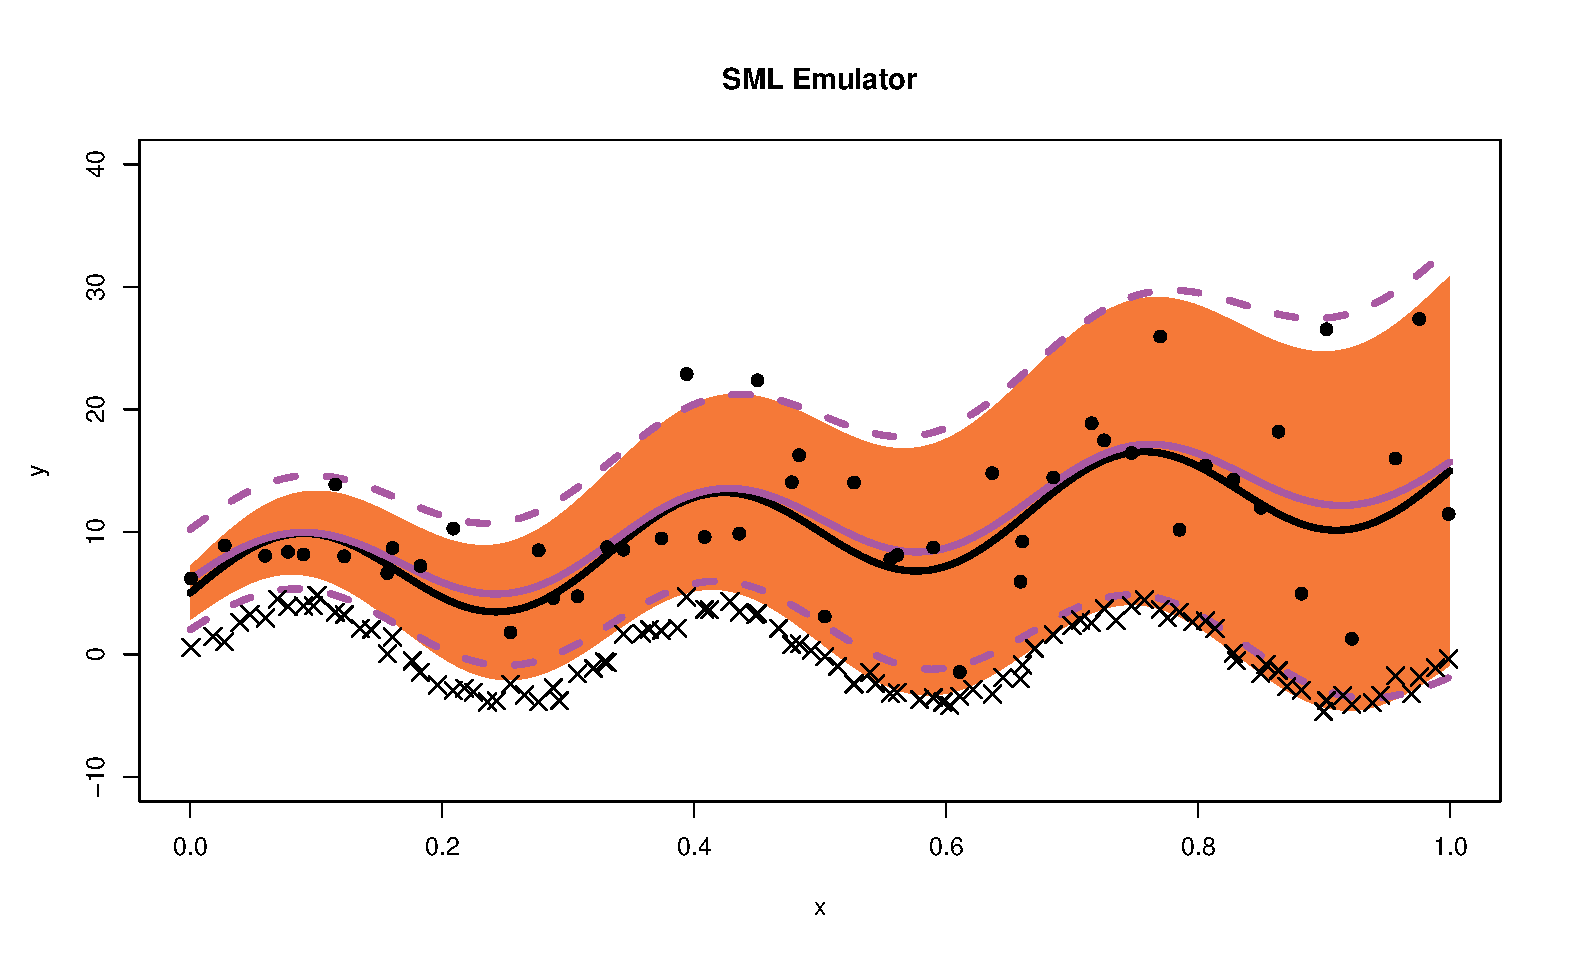
\includegraphics[width=0.75\textwidth]{sml-het-fig/sml-example.eps}
	\caption{SML emulator using design (b) ($49$ expensive runs and $100$ cheap runs). Expensive runs are the black points and the cheap runs are black crosses. True simulator represented by the black line (mean function) and orange band ($\pm 1.96$ standard deviations). Emulator represented by purple line (emulator mean) and dashed purple lines ($\pm 1.96$ emulator standard deviations).}
	\label{Fig:comparison}
\end{figure}

\section{Stochastic Multilevel Emulation of the Athena Simulator}

We return to the motivating example for the SML emulator; the Athena model. Athena is a large point-process model. Simulations are implemented via MATLAB with a large number of inputs. Many inputs are parameters of lifetime distributions of components in wind turbines, but others, for instance, relate to the availability of repair equipment. These additional inputs are not considered here; we are interested in the component reliabilities which are most critical to offshore wind farm availability.

\subsection{Emulator Construction}

We construct emulators over a $9$ dimensional input space. These inputs are the expected lifetimes of key wind farm components: gearbox, generator, frequency converter, transformer, main shaft bearing, the blades, tower, foundations and the catch all. We vary each input over the range $[0.1, 5]$ (years). In the Athena model, each turbine (and subassembly within the turbine) can have its own unique parameters, we give the same parameters to each subassembly of a given type and allow different types of subassembly to have different values. However, each turbine will fail independently of other turbines. The design points are chosen via the structure described in \Cref{Sec:design}. To construct the HetGP emulator we ran the simulator at $100$ design points, with simulator runs taking, on average, $11$ minutes each. The cheap runs of the simulator were fast enough that we could trade just $5$ expensive design points for $495$ cheap runs. We used mean functions $m_E(\bx) = (1, \log(x_1), \ldots, \log(x_9))\bm{\beta}_E$ and $m_C(\bx) = (1, \log(x_1), \ldots, \log(x_9))\bm{\beta}_C$.  However, for the covariance function, we standardise the inputs by subtracting the sample means and then dividing by the sample standard deviations (of the expensive training data). These transformed inputs are denoted $x_i^*$. The latent variance GP has mean function $m_V(\bx) = (1, \bx^*)\bm{\beta}_V$ and again, the covariance function assumes standardised inputs.

\begin{figure}
	\centering
	\includegraphics[width=0.7\textwidth]{sml-het-fig/obs-pred.pdf}
	\caption{Observed probit availability (training data) plotted against emulator mean predictions (black dots) and $500$ realisations from the emulator at each point (translucent red circles).}
	\label{Fig:within-sample}
\end{figure}

\Cref{Fig:within-sample} shows the emulator predictions of the probit training points with realisations from $\mathcal{N}\{m^*(\bx), V^*(\bx)\}$ around each prediction. We can see that large deviations from the unit diagonal are typically accompanied by a more diffuse predictive distribution; the emulator is giving larger variance to the points which are far away from the mean. We also see that the observed probit availabilities are mostly in the region of $1.5$ -- $2$ (availabilities in the region of around $0.93$ -- $0.97$). The full range of observed availabilities is $(0.762, 0.980)$, the vast majority of realisations from the emulator agree with this range.

Using $100$ independently generated validation data points, the MSE (on the probit scale on which the emulator was constructed) for HetGP was $0.0315$ whereas SML achieved an MSE of $0.0272$. The score for HetGP was $166$ and for SML the score was $254$ (again, on the probit scale). Since we transformed the availability to construct emulators on an unbounded space, we should also check how predictions perform on the original scale (transforming back to values in the range $(0,1)$). Using an inverse-probit transformation on the mean function provides a sensible point estimate of availability. Comparing the MSE on the original scale  we observe an MSE of $6.00\times 10^{-4}$ for HetGP, and under SML the MSE is reduced to $4.66\times 10^{-4}$. Hence, SML achieves better MSE and score here than HetGP for the Athena model, suggesting it is a better emulator. Further, our MAP estimate of $\rho$ is $\hat{\rho} = 0.63$, suggesting that the cheap version of the Athena simulator is moderately correlated with the more expensive version, despite the different wind farm topologies.%KJW: a 'picture' of the emulator?

\subsection{Emulator Validation}

In order to check the validity of the emulators, we will implement some of the graphical diagnostics proposed by \citet{Bastos09}. Since we model the (transformed) simulator outputs by a Gaussian process, the Cholesky errors (CEs) should form a random sample from a $\mathcal{N}(0, 1)$ distribution (approximately). If the posterior mean and variance are well suited to the simulator, the validation data should lie in a horizontal band, centred at $0$, with approximately $95\%$ of points in the interval $(-1.96, 1.96)$. We can also compare empirical quantiles of the CEs against theoretical quantiles -- we do this via coverage plots which compare the proportion of CEs in the $100(1-\alpha)\%$ prediction interval against the expected proportion.
\begin{figure}[!h]
    \centering
    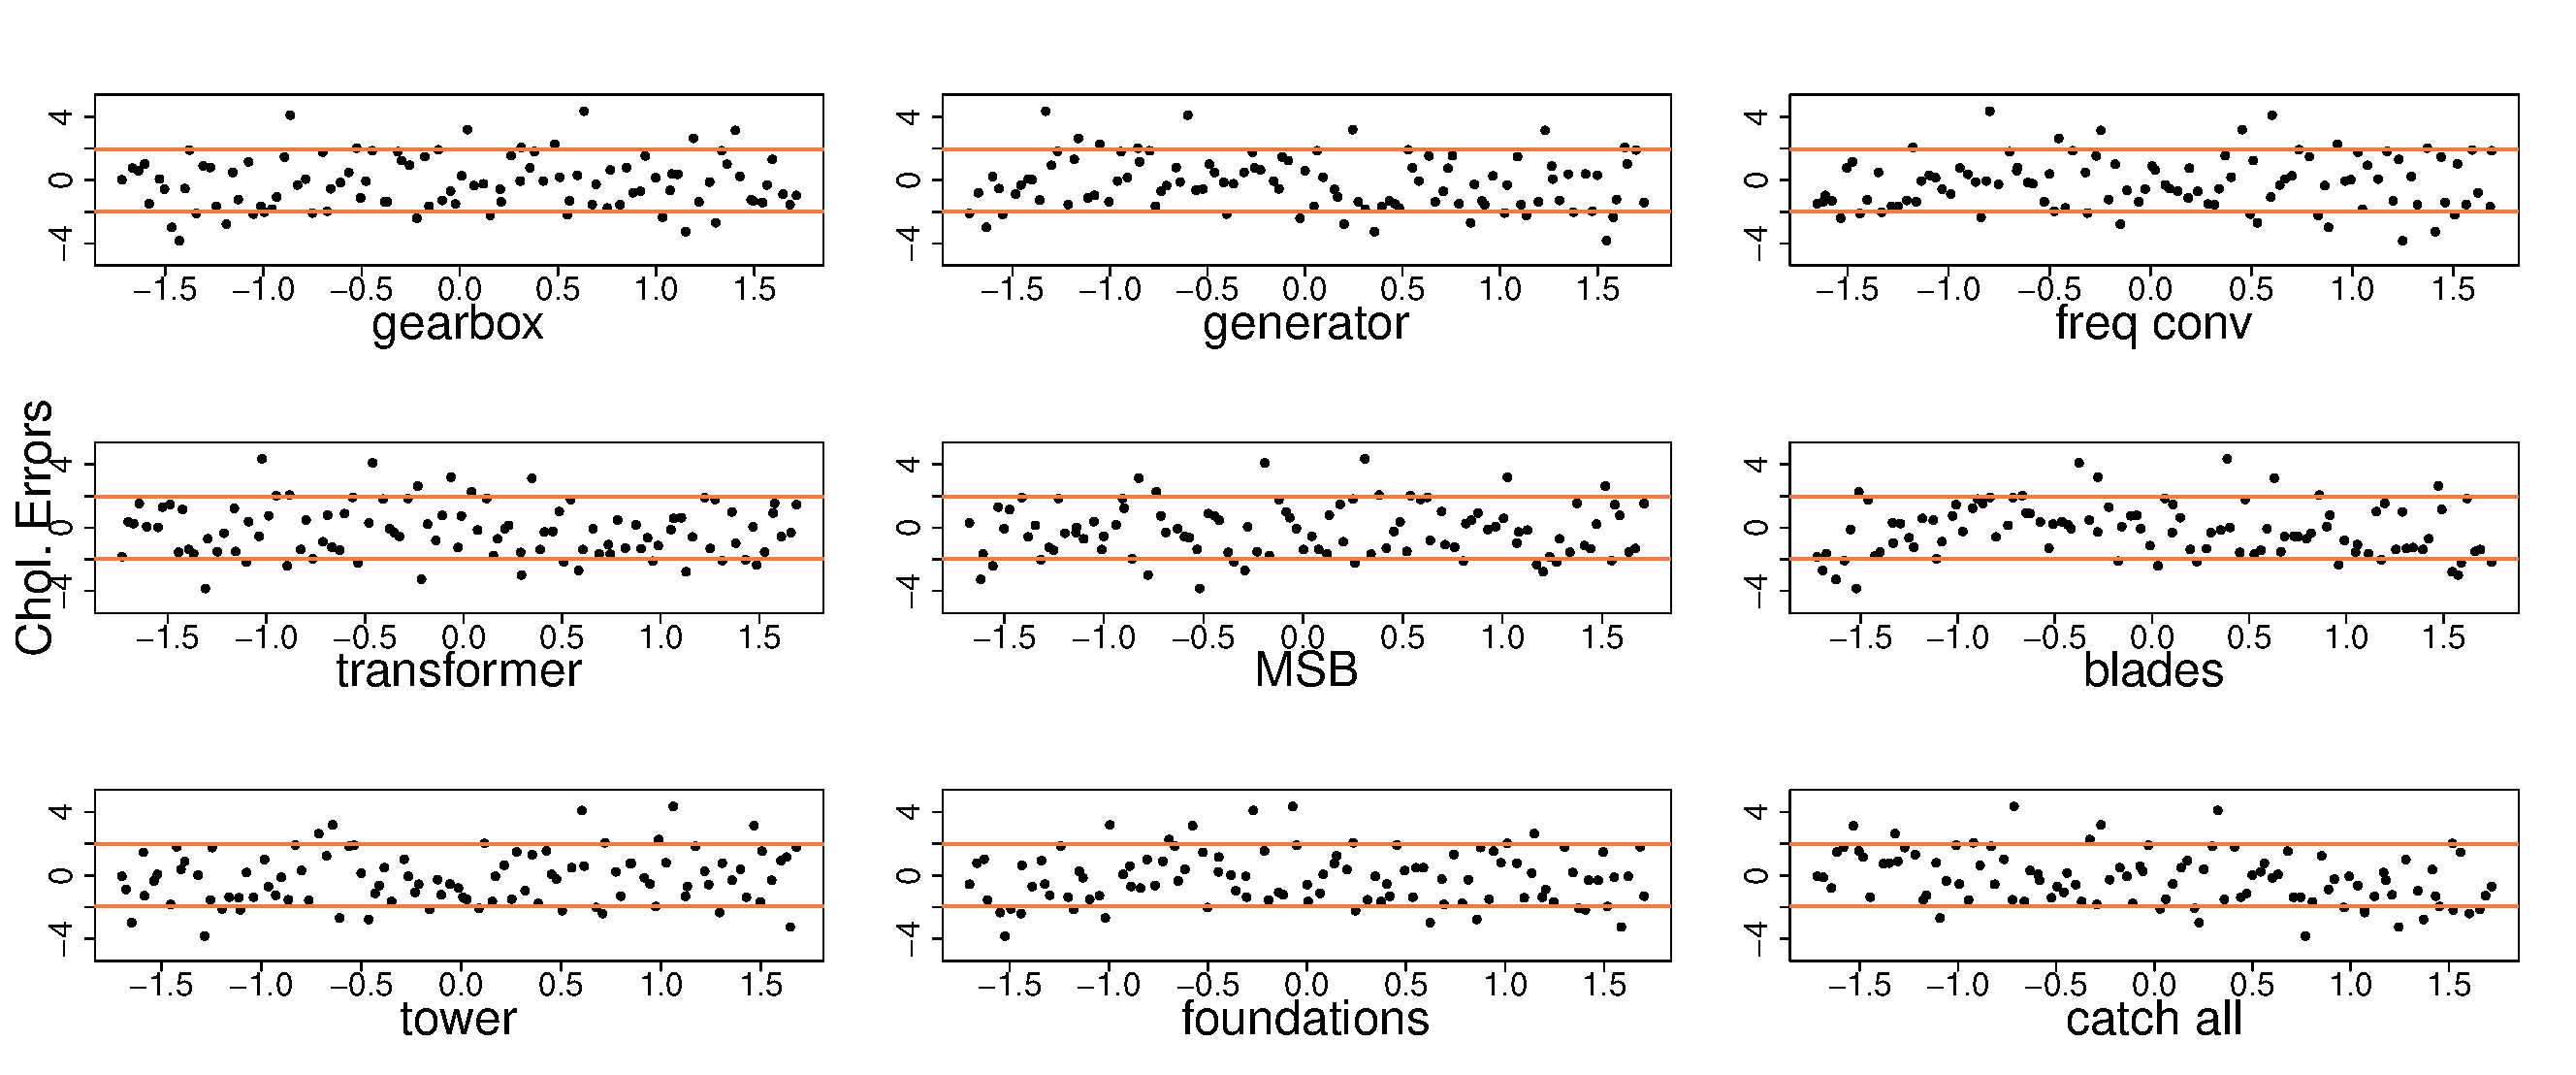
\includegraphics[width = 0.8\textwidth]{sml-het-fig/het-resids.eps}
    \caption{Cholesky errors for HetGP, based on $100$ ``unseen'' validation points. The $x$ axis is on the standardised scale and orange lines are at $\pm 1.96$.}
	\label{Fig:het-resids}
\end{figure}
\begin{figure}[!h]
    \centering
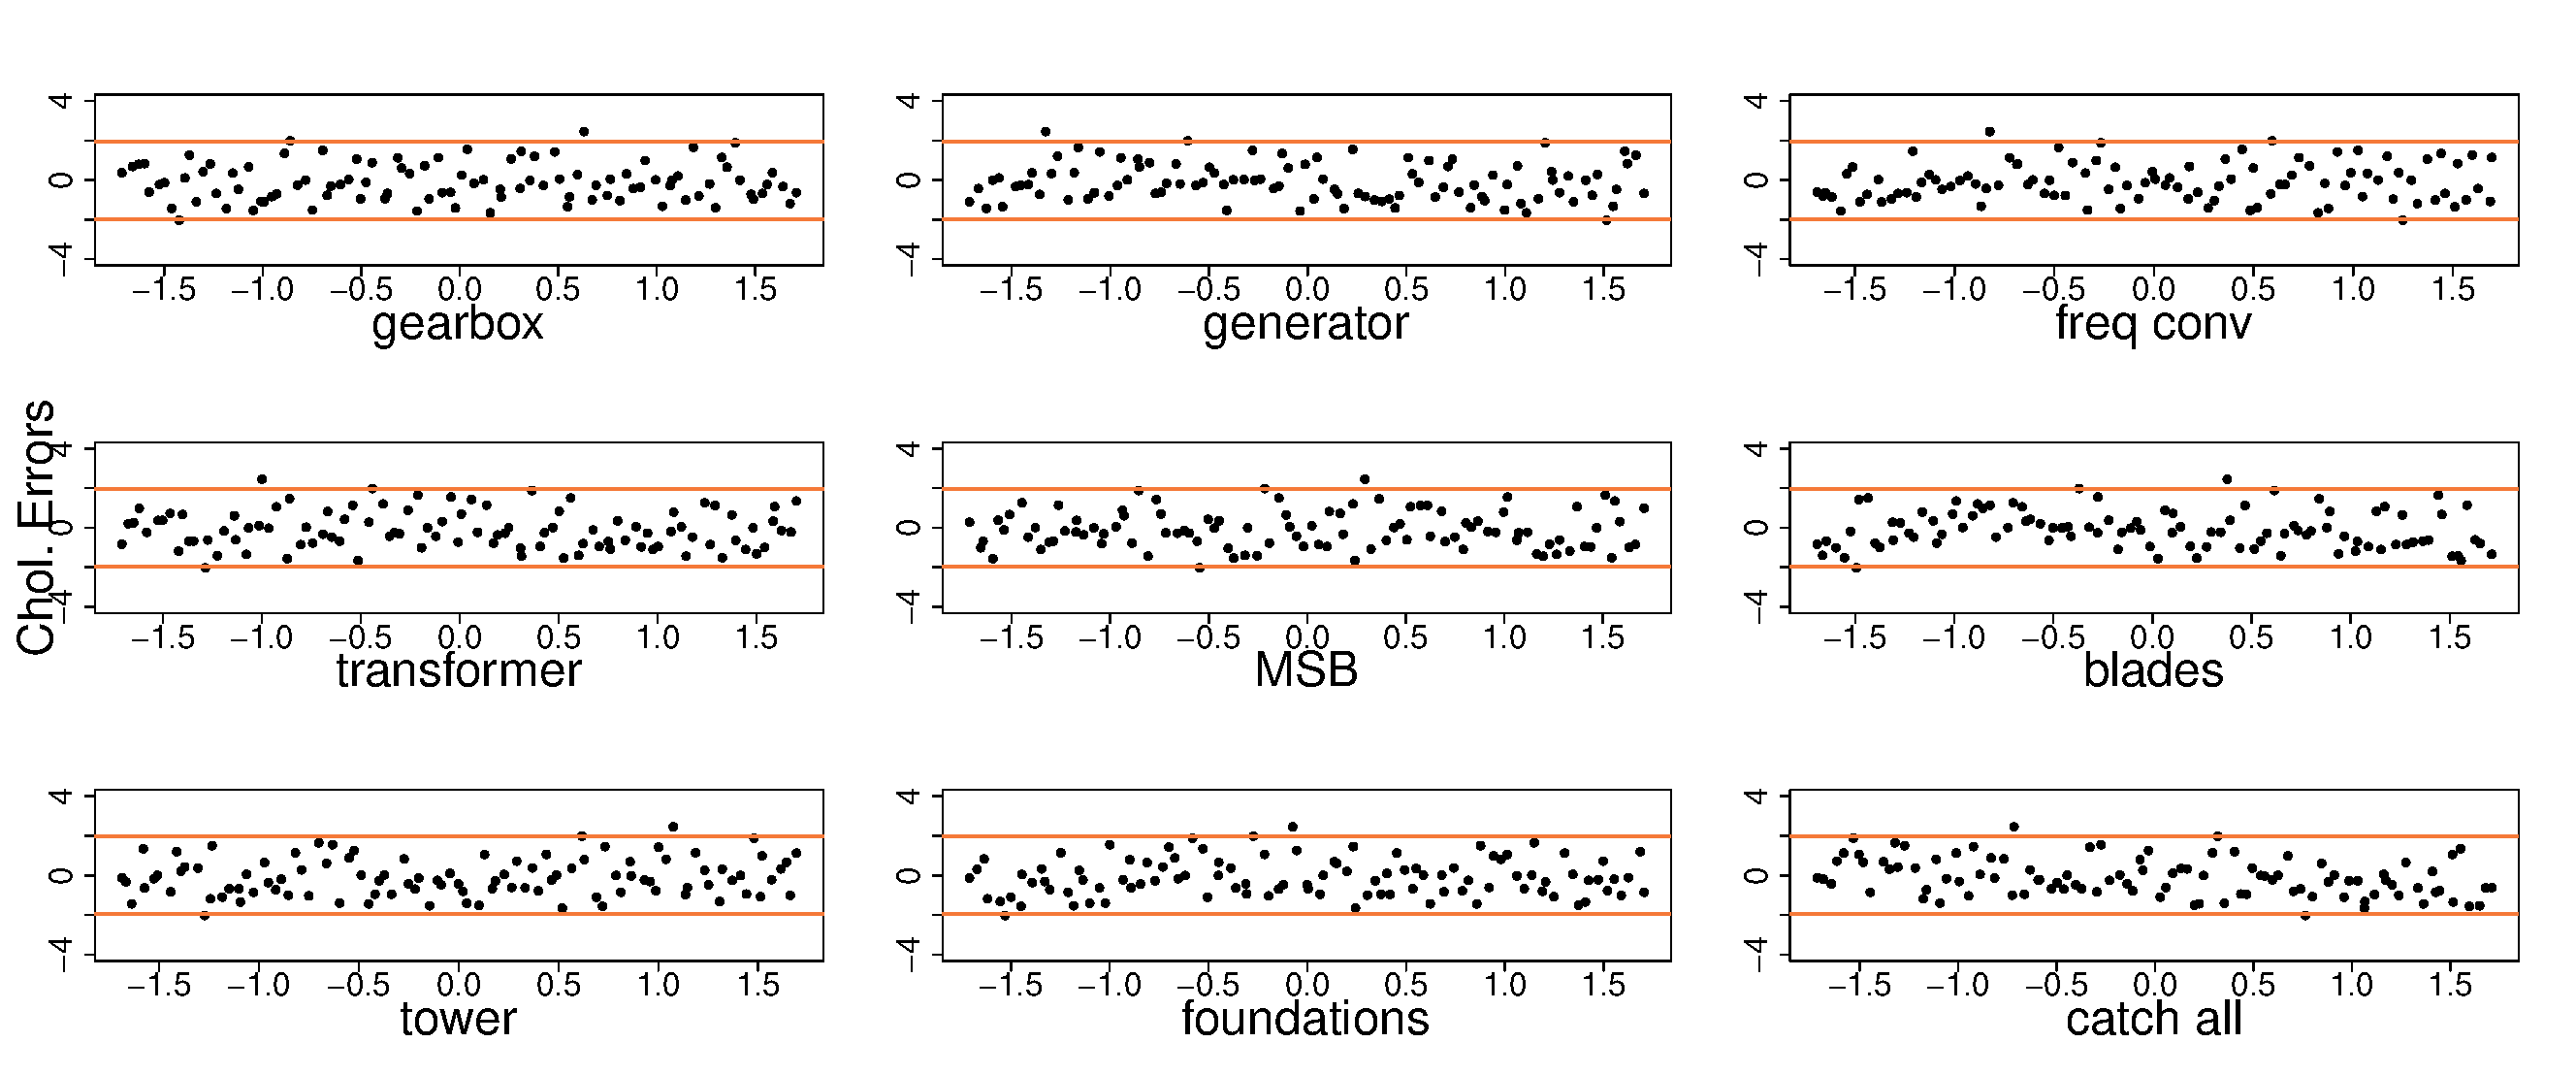
\includegraphics[width = 0.8\textwidth]{sml-het-fig/sml-resids.eps}
    \caption{Cholesky errors for SML emulation, based on $100$ ``unseen'' validation points. The $x$ axis is on the standardised scale and orange lines are at $\pm 1.96$.}
	\label{Fig:ml-resids}
\end{figure}
\begin{figure}[!h]
    \centering
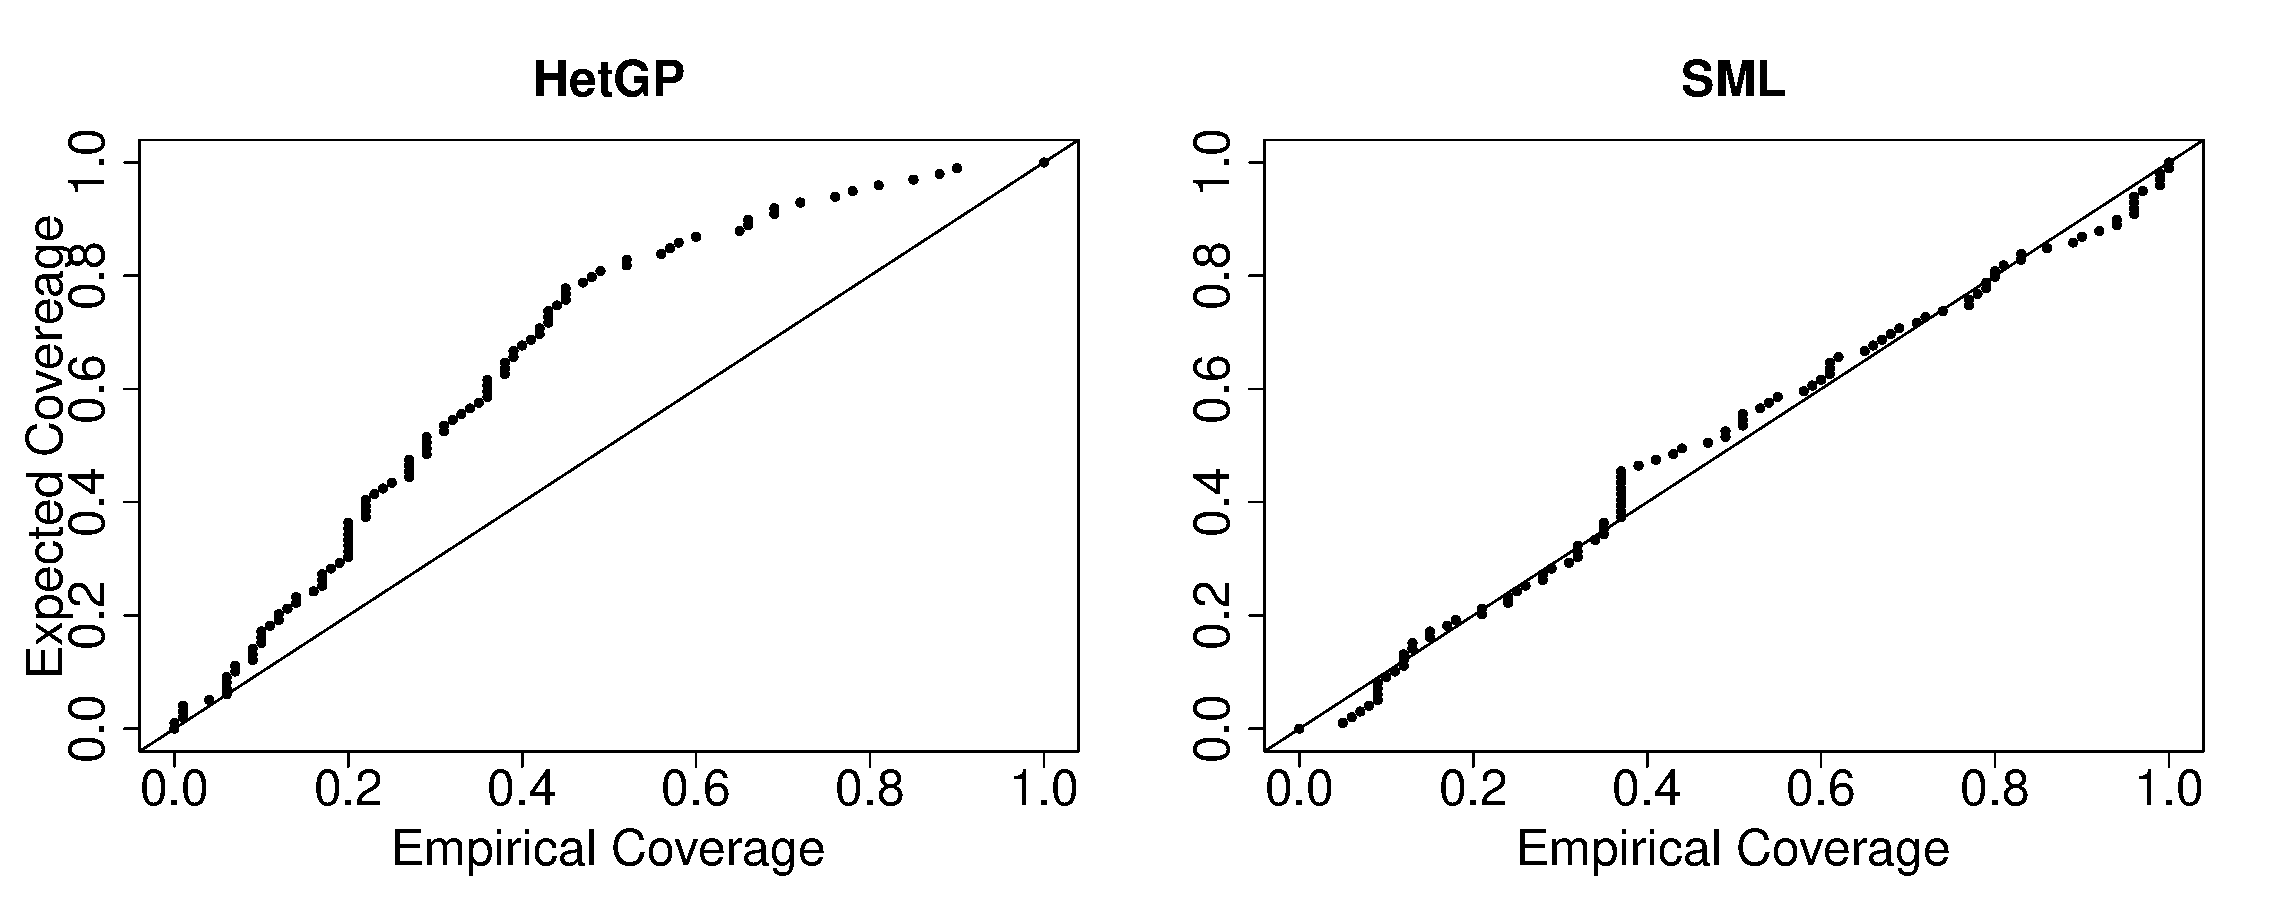
\includegraphics[width = 0.7\textwidth]{sml-het-fig/coverage.eps}
    \caption{Out of sample coverage plots, using the Cholesky errors of the ``unseen'' validation data.}
	\label{Fig:coverage}
\end{figure}

We see in \Cref{Fig:het-resids} that the magnitude of CEs for HetGP can be very large, whereas for SML the points appear to be a random $\mathcal{N}(0,1)$ sample. Far more CEs than we would expect are outside the range $(-1.96,1.96)$: $22 \%$. For SML (\Cref{Fig:ml-resids}), $3\%$ of CEs are outside of $(-1.96,1.96)$, just under the expected $5\%$; an improvement over HetGP. The coverage plots also show that the Gaussian assumption is more plausible for the SML emulator than HetGP; the empirical overage is close to the expected coverage under SML. The HetGP emulator's coverage quickly deviates from the expected coverage, and the empirical coverage is almost always much less than the expected coverage.

\section{Probabilistic Sensitivity Analysis of Athena}

We will now use the SML emulator to perform efficient PSA on the Athena simulator. We want to deduce which of the inputs are the ``driving force'' of the output uncertainty to help us best plan a probability elicitation. Since our simulator of interest is stochastic, we utilise the approach of \citet{Marrel2012}, using the posterior mean of the GP as a plug-in estimate for the simulator's expected value. Similarly, we use the posterior mean value of the log-variance process as a plug-in estimate. The sensitivity analysis we perform will be on the probit-availability scale (the scale the emulator was constructed on). We will illustrate the necessary mathematical details here for stochastic PSA. Details for the deterministic case can be found in \cite{Oakley04}.

\subsection{Stochastic PSA}

A deterministic simulator can be thought of as a map $\eta: \R^K \to \R$ with $\bx \mapsto y = \eta(\bx)$. A stochastic simulator can also be thought of as a map $\eta: \R \times \N \to \R$ with $(\bx, x_\varepsilon) \mapsto y = \eta(\bx, x_\varepsilon)$ where $\bx$ are the simulator inputs and $x_\varepsilon$ is the seed used for the simulator's random number generation scheme.

It is also useful to think of the stochastic computer model as a mean function $Y_m(\bx) = \E(\eta(\bx)|\bx)$ and a dispersion function $Y_d(\bx) = \var\{ \eta(\bx)| \bx \}$. Our GP assumptions make higher order moments redundant. Then the total uncertainty in the stochastic computer model output is, by the total variance formula,
\begin{equation*}
V = \var(Y) = \var\{Y_m(\bx) \} + \E\{ Y_d(\bx) \}
\end{equation*}
where the expectations and variances are taken over $\bx$.

The mean response has an ANOVA decomposition into main effects and interactions:
\begin{equation*}
Y_m(\bx) = f_0 + \sum_i f_i(x_i) + \sum_{i<j} f_{ij}(x_i, x_j) + \sum_{i<j<k} f_{ijk}(x_i, x_j, x_k) + \cdots + f_{1\ldots K} (\bx),
\end{equation*}
where $f_0 = \E \{ Y_m(\bx)\} $, the expected simulator output (again, expectation taken with respect to $\bx$), $f_{ij}(x_i, x_j)$ is the first order interaction between variables $i$ and $j$, $f_{ijk}(x_i, x_j, x_k)$ denotes the interaction between variables $i$, $j$ and $k$ and so on. We then compute the main effects and first order interactions by
\begin{align*}
f_i(x_i) &= \E \{ Y_m(\bx) | x_i \} - f_0\\
f_{ij}(x_i, x_j) &= \E \{ Y_m(\bx) | x_i, x_j \} - f_i(x_i) - f_j(x_j) -f_0.\label{Eq:interact}
\end{align*}
Higher order interactions terms, $f_J(\bx_J)$ for any $J \subseteq \{1, 2, \ldots, K \}$,  can be found in a similar way.
The observed response (accounting for stochasticity) is
\begin{equation}
\eta(\bx) = Y_m(\bx) + f_{\varepsilon}(\bx) + \sum_{  J  \subseteq \{1, \ldots , K\} } f_{ \varepsilon J}(\bx) \label{Eq:observed}
\end{equation}
where $f_\varepsilon (\bx)$ is the main effect of the seed and $f_{\varepsilon J}(\bx)$ is the interaction between the seed and the variables attributed to subset $J$.

We can use the main effects and interactions to determine how much of the uncertainty in $Y_m(\bx)$ is attributed to a particular subset of the inputs $J \subseteq \{1, 2, \ldots, K\} $,
\begin{equation*}
	V_J = \sum_{J' \subseteq J} \var \{ f_{J'} (\bx_{J'}) \}.
\end{equation*}
Normalising these variances by $V$ gives us a scaled quantity $S_J = V_J / V \in [0,1]$ which is the proportion of variance in $Y$ induced by the uncertainty in $\bx_J$. However, in the stochastic setting, $S = \sum_{i} S_i + \sum_{i<j} S_{ij} + \ldots + S_{1\ldots K}  =\var \{ Y_m(\bx)\} / V  < 1$. The remaining uncertainty is accounted for by
\begin{equation*}
S_{T_\varepsilon} = \frac{ \E \{Y_d(\bx)\} } {V}
\end{equation*}
which is the total uncertainty induced by the random seed. This is the proportion of uncertainty attributed to the terms with an $\varepsilon$ subscript in \Cref{Eq:observed}; it can be thought of as the ``uncontrollable'' uncertainty in the computer experiment.

\subsection{Application of PSA to Athena using the SML emulator}

To estimate all the above quantities, we replace the Athena simulator, $\eta(\cdot)$, with the SML emulator, $\hat{\eta}(\cdot)$, constructed above. We estimate all relevant quantities by Monte Carlo simulation to compute the expectations and variances with respect to $\bx$, conditional on all GP parameters. It is common in PSA to give a simple probability distribution to the inputs of interest \citep{Kennedy2006,Saisana2005,Overstall2016}. Although these probability judgements are a bit rough and ready, they are sufficient for the problem at hand \citep{Ohagan2019}. Our parameters are each assumed to follow $U(0.1, 5)$ distributions, which covers the range for which the emulators were constructed. We sample many thousands of such random variables and propagate them through $Y_m(\cdot)$ and $Y_d(\cdot)$ to compute the main effects and their associated sensitivity indices. Estimated first order sensitivity indices are given in \Cref{Table:first-order}. The largest two account for over $80\%$ of simulator output, they are the generator ($\hat{S}_2 = 25.36\%$) and the blades ($\hat{S}_6 = 55.86\%$). We also estimate $\hat{S}_{T_\varepsilon} = 4.49$, suggesting that the uncontrollable uncertainty is relatively low compared to the variation in simulator output. The proportion of uncertainty amongst all possible interactions amongst controllable variables is $6.27\%$. The largest three second order terms are $\hat{S}_{2,6} = 1.06\%$ (generator/blades), $\hat{S}_{3,6} = 0.84\%$ (frequency converter/blades) and $\hat{S}_{5,6} = 0.70\%$ (main shaft/blades), all of which are linked to the blades of the turbine (input $6$). However, all but one of these interaction terms accounts for under $1\%$ of output variance, suggesting the Athena model is approximately additive in the mean response. Quite clearly this indicates that failures in turbine blades are most critical to maintaining high availability. This is also seen in \Cref{Fig:main-effs}; the (mean centred) main effect plot shows $f_6(x)$, the main effect of the blades as being the most prominent effect, followed by $f_2$ the main effect of the generator, with all other variables having similar amounts of variability, agreeing with the estimated values of each $S_i$.
%% insert table
\begin{table}[h]
	\centering

\begin{tabular}{@{}clr@{}}
    \toprule

	$i$ & Subassembly & Main effect ($\hat{S}_i$)\\\cmidrule{1-3}
	$1$ & Gearbox & 0.07\\
	$2$ & Generator & 25.36\\
	$3$ & Frequency converter & 0.20\\
	$4$ & Transformer & 0.79\\
	$5$ & Main shaft bearing & 0.64\\
	$6$ & Blades & 55.86\\
	$7$ & Tower & 1.37\\
	$8$ & Foundations & 0.13\\
	$9$ & Catch all & 4.42\\\bottomrule
  \end{tabular}
	\caption{Estimated first-order sensitivity indices (expressed as a percentage) for the Athena simulator, with computation facilitated by SML emulator.}
\label{Table:first-order}
\end{table}
\begin{figure}[h]
\centering
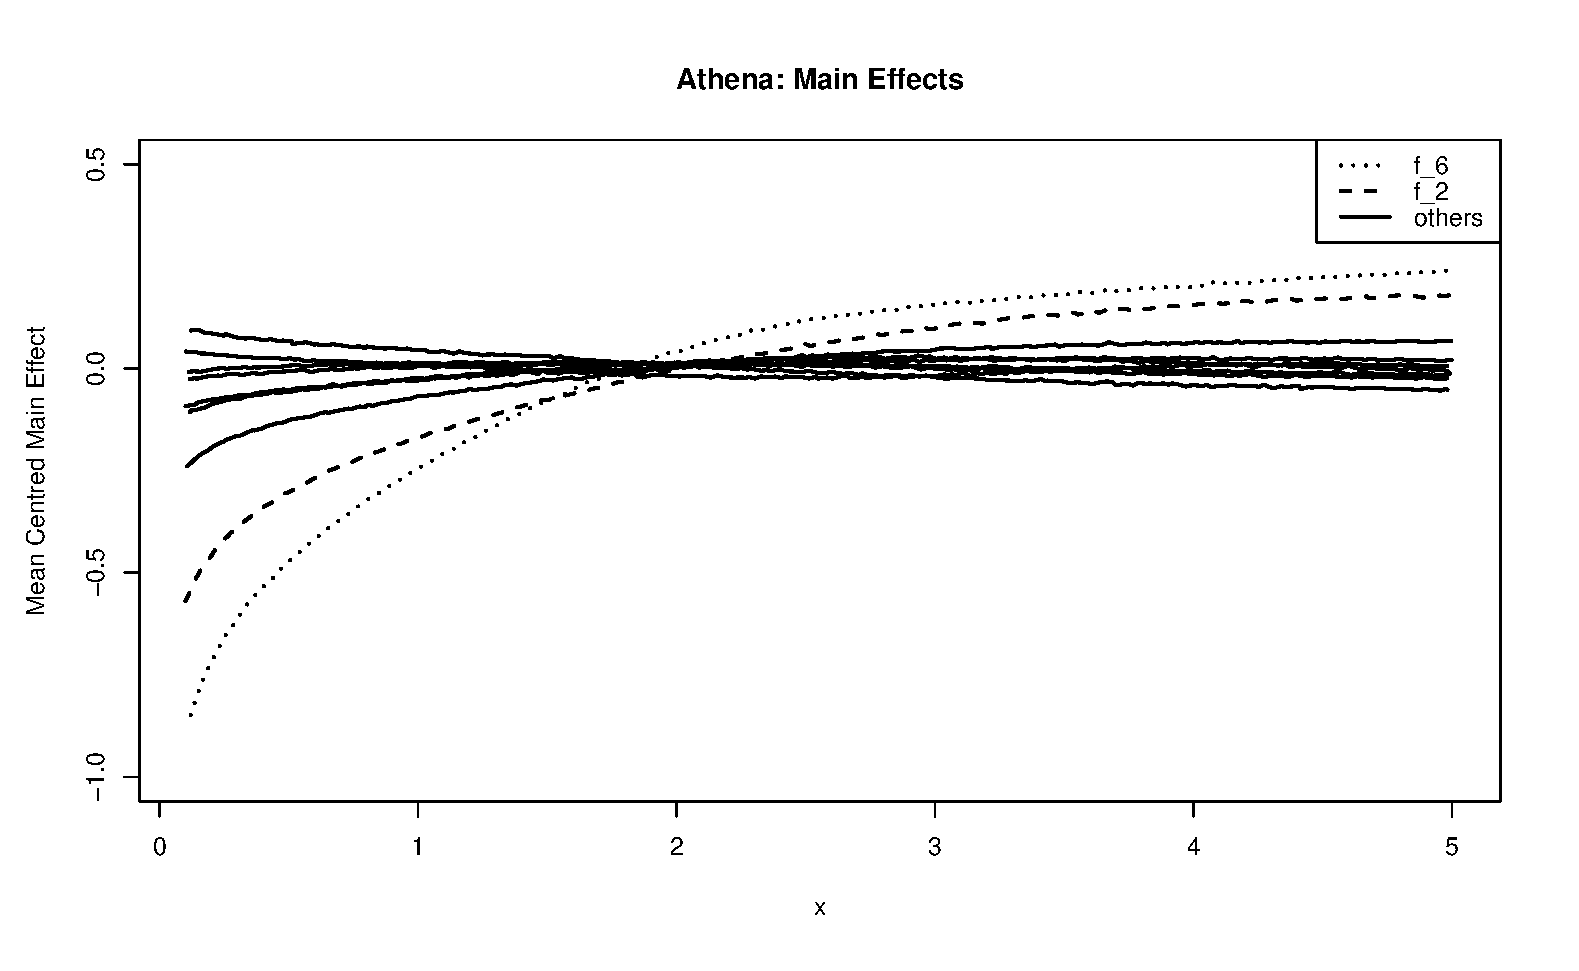
\includegraphics[width=0.8\textwidth]{sml-het-fig/main-eff-mono.eps}
\caption{Mean-centred main effects plotted for the $9$ inputs, on the probit-scale. Dotted line corresponds to $f_6(x)$ (blades) and dashed line to $f_2(x)$ (generator). Solid lines represent the main effects all other variables, each of which have individual variance contribution $<5\%$.}
\label{Fig:main-effs}
\end{figure}

We have now performed the necessary analyses to set up our elicitation procedure; our largest contributions to output uncertainty were the failures of the blades and generator. Our planning of the `full' elicitation of parameters would focus mainly on these two parameters, since they jointly contribute to over $80\%$ of output uncertainty. Without an emulator this analysis would have taken many months of CPU time. Our SML emulator allowed us to further reduce the amount of time required to construct an adequate emulator by exploiting a computationally cheaper version of the Athena simulator.
%\clearpage
\section{Conclusions \& Further Work}
%We have constructed an appropriate emulator of the Athena simulator using a novel multilevel approach, extending the methodology of \cite{Kennedy2000} to the stochastic case. Our emulator has allowed us to perform an efficient sensitivity analysis to understand the influence of parameter uncertainty on output uncertainty, allowing a practicioner to explore the impacts of decisions on wind farm performance.
We have introduced a stochastic multilevel emulator which adopted elements of the autoregressive structure from \cite{Kennedy2000} to construct a more accurate mean function and the latent variance structure of HetGP to account for a heteroscedastic computer model. This structure allowed us to link together two versions of the Athena simulator to perform accurate and efficient sensitivity analysis. The easy to generate training data allowed us to build an adequate emulator without having to spend many days generating training data.

It would be interesting to see, from a methodological point of view, how the SML emulator could be improved. One idea would be to implement a sequential design rule similar to that of \citet{Gratiet2015}. It would also be interesting to see if replicates could improve this type of emulator in the same way that replicates benefit HetGP. Replication could be especially beneficial in the cheap simulator; this would help to reduce the size of computational overheads of a large design matrix (although our design matrix for the Athena emulator was not particularly large). Another possibility would be to link the variance of the two simulators; we chose not to do this as it would involve linking two latent variance processes and would involve inversion of a large matrix, increasing the computational cost of inference and prediction.

A detailed probability elicitation can be very useful in the event of limited data, such as our wind farm setting. Although there is a large amount of data from existing wind farms, this is not directly relevant to a future wind farm so should not be blindly applied to the problem of planing a future wind farm. We would focus on the most important parameters to reduce the burdens associated to probability elicitation, these were found to be the expected lifetime of the generator and the blades, so the bulk of our effort would be spent on the elicitation of these parameters. This also tells us that we could reduce the dimension of the problem; five of the parameters had first order indices estimated to each be under $1\%$. It could be considered adequate to condition on likely values for these parameters to further focus on the uncertainties most critical to the problem at hand.

Our ultimate goal is to utilise an emulator of the Athena simulator in a Bayesian decision analysis to allow a Decision Maker to answer questions concerning the design and maintenance strategy of large offshore wind farms. This would involve eliciting a utility function over availability and other features such as, but not limited to, the monetary cost of particular turbine components.

\end{chapter}
